\chapter{LLHD and MLIR}
\label{ch:ir}

%---------------------------------------------------------------------------------------------------

\section{LLHD}
\label{section:llhd}
The Low-Level Hardware Description (LLHD) language \cite{Schuiki2020, llhd.io}, is a novel Intermediate Representation (IR) targeted at hardware design. This heavily LLVM inspired IR has a simple and contained instruction set, yet is powerful enough to represent designs coming from well established Hardware Description Languages (HDL), such as SystemVerilog \cite{SV2018} and VHDL \cite{VHDL2009}. Together with the language definition comes a SystemVerilog compiler frontend, \texttt{moore} \cite{moore}, as well as a reference simulator \cite{llhd-sim}, all implemented in \textit{Rust}.

%-------------------------------------------------------------------------------

\subsection{The Language}
The LLHD language takes the form of a Multi-level Single-Static-Assignment (SSA) \cite{Alpern1988} language, specifically tailored to represent hardware design flows in their entirety.
One of the core differences that takes LLHD apart from conventional, software-targeted IRs, is a first class notion of passing time. This is achieved through a type, \texttt{time}, composed of three distinct elements:

\begin{itemize}
    \item a \textit{real-time} value, describing an amount of time (\eg, in seconds or nanoseconds),
    \item a \textit{delta step} value, describing an infinitesimal time step inside a real-time step,
    \item and an \textit{epsilon step} value, describing an absolute time slot within a delta step.
\end{itemize}

This construct allows to clearly define the order of events in a design, which is required for behavioral simulation.

Another core difference, closely related to the time type, is the \texttt{signal} type. This is used to describe physical signals, or wires, carrying some value. A signal can be accessed through a \textit{probe}, and updated through a \textit{drive}, representing a parallel to pointers to memory locations in conventional programming languages (such as \textit{C/C++}), where storing a new value takes some predefined (time) delay. This is used to model the propagation delays of signals in a physical circuit, and enables the persistence of values across time steps.

A hardware description also requires to model the structure and hierarchy of a design. This is accomplished through three modeling constructs, called \textit{units}:
\begin{itemize}
    \item \textit{Entities} provide a structural circuit description, as well as a notion of reuse and concurrency. They define a list of instructions executed in a timed data-flow fashion and build the structure of the design by creating signals and instantiating other units, which operate concurrently.
    \item \textit{Processes} provide a behavioral circuit description. They define a list of basic blocks and instructions and are thus governed by (timed) control-flow. In addition to the conventional branching operations, processes can suspend their execution, either for a given amount of time, or until a specific signal changes, or both. Also, important to note is that they cannot define new signals or instances, in opposition to entities.
    \item \textit{Functions} provide a notion of code reuse and recursion. They correspond to the conventional notion of functions, \ie, a mapping between a set of input values and zero or one output values, but don’t have a physical equivalent. Similar to processes, they are governed by control-flow and define a list of basic blocks and instructions. Though, differently from the other two units, they execute immediately, and cannot contain any delayed operations.
\end{itemize}

\mlirfile{A simple LLHD design.}{A simple LLHD design containing a root entity, which defines a signal and instantiates a basic process, toggling a boolean signal back and forth each nanosecond, until the end of time.}{llhd_toggle}

Circuit designs in HDLs generally model circuits both behaviorally and structurally. Behavioral descriptions, though, are mere verification and simulation constructs, which do not have a physical equivalent. For this reason, one IR is not enough to fully represent designs coming from HDLs. LLHD addresses this by defining three distinct levels of abstraction (or \textit{dialects}), each being a strict subset of the previous one.

At the base, we have the \textit{netlist} level, which only contains entities and signals. This describes the design at a netlist level, the result of synthesis. Next, we have the \textit{structural} level, which represents a design in a pure structural way, or the relation between inputs and outputs. At this level, only entities are present, and the resulting code is fully synthesizable. On top, we have the \textit{behavioral} level. This contains the full LLHD instruction set and introduces the non-synthesizable simulation and verification constructs required to fully represent designs coming from HDLs.

%---------------------------------------------------------------------------------------------------

\section{MLIR}
\label{section:mlir}
The Multi-Level Intermediate Representation (MLIR) \cite{Lattner2020} is a novel approach at building compilers. It defines a modular and extensible IR, composed of \textit{dialects}, which can be freely defined by users. It comes with an extensive infrastructure that allows defining new dialects, passes, and analysis with relative ease, aiming at reducing the cost and redundancy of building new domain-specific compilers and IRs.

%-------------------------------------------------------------------------------

\subsection{Operations}
\label{section:mlir_ops}
The main unit of semantics in MLIR is an Operation (in short \textit{Op}). Ops are used to model everything, ranging from instructions to functions, to modules.  They can define regions (one or multiple), take SSA operands as arguments, define new SSA operands as results, and may also have attributes or location information attached to them. MLIR does not provide a fixed set of operations, but rather strongly encourages user-defined extensions.

New operations are usually defined through the Operation Definition Specification (\textit{ODS}) framework, an LLVM \textit{TableGen} \cite{tablegen} extension which allows defining operations, as well as generating specialized \textit{C++} classes in a descriptive fashion, cutting down in the redundancy introduced by the boilerplate code required to define new operations, as well as aiming at reducing errors due to sub-optimal coding practices. Most operations do not require any additional coding, while more complex ones require some additional \textit{C++} fiddling, most notably operations containing regions.

SSA operands, as per convention, are labeled through a \texttt{\%} character, followed by some identifier string. In MLIR, operand names don’t carry any semantic meaning. They can thus not be queried for their name, and name generation is hidden from the user and handled by the MLIR infrastructure. The default operand name is just a number, while in some exceptional cases where the value is statically known, a more descriptive name is generated (notably for constant-like operations, \eg \texttt{c42\_i12} for an \texttt{i12} constant with value 42). The rationale is that usually, an SSA operand does not carry any relevant information, and making the infrastructure manage SSA ID generation makes both the textual representation more readable and extension easier, as they do not need to be considered.

MLIR provides a generic text representation for Ops, which is automatically available to all operations. Operand \texttt{\%0} in Listing \ref{listing:custom_op} shows the format of MLIR's generic syntax, where we can always find the operation name first, printed in string format (\ie, enclosed in quotation marks), followed by a list of operands enclosed in parentheses. A list of attributes (the \textit{attribute dictionary}, or \textit{attr-dict}) follows, enclosed in curly brackets. Finally, the argument and result types are printed in functional form after a colon.

A custom syntax can be defined by the user, to give a more human-readable representation, either through TableGen (for simple operations) or by defining a custom printer/parser pair. Operand \texttt{\%1} in Listing \ref{listing:custom_op} shows a possible custom syntax for our custom operation, where the attribute has been moved in the first position after the operation name, and the parenthesis have been removed from the functional type annotation.

Important to note is that in both generic and custom syntax, the operation name's format is statically assigned, meaning that it will always have the form “\textit{dialect.op\_name}“. When a custom syntax is defined, the quotation marks around the name are also automatically dropped.

\mlirfile{A MLIR custom operation.}{A simple example of a custom operation's generic syntax (\texttt{\%0}) and a possible custom syntax (\texttt{\%1}).}{custom_op}

%-------------------------------------------------------------------------------

\subsection{Types and Attributes}
\label{sec:mlir_types}
Like LLVM, every MLIR SSA operand has a type attached to it. A standardized set of the most commonly used types is provided by the infrastructure, in the built-in dialect. Included are types such as variable bit-width integers and floating-point (e.g. \texttt{i1}, \texttt{i32}), function types and tuples. Also, user-defined types can be defined as part of a new dialect.

Attributes in MLIR represent constant values known at compile-time, such as numeric values, strings, or symbols. Similar to types, MLIR provides a standard set of attributes for the most commonly used types, but user-defined attributes can also be introduced.

Different from operations, there is currently no declarative way to define types and attributes, and they have to be implemented as \textit{C++} constructs.

%-------------------------------------------------------------------------------

\subsection{Regions and Blocks}
MLIR provides a nesting structure through regions. An Op might have one or more regions attached to it. A region then consists of a list of blocks, and a block consists of a list of instructions, which always terminates with an operation known to be a terminator. The only exception is for operations with a specific trait, which marks them as having only a \textit{single block with implicit terminator}. Here the terminator and block label of the first (and only) block can be omitted, and the well-formedness of the operation is ensured by the operation parser.

Instead of using $\phi$ nodes, MLIR uses block arguments, \ie, a block can define a (potentially empty) list of arguments, similar to a function. Terminators assume the role of a caller, passing correct-typed SSA operands when branching to a block.

The visibility of values is determined by the SSA \textit{dominance condition} (\ie, a value has to be defined before it's \textit{use} in the Control-Flow Graph) and the nesting and semantic properties of enclosed operations. An operation within a region is thus not allowed to use values lexically defined after the region but can access values preceding it. This property can be disabled by marking an operation as \textit{isolated from above}, effectively blocking it from accessing operands defined outside its region. Inside regions and blocks, SSA dominance has otherwise always to be satisfied.

MLIR also offers \textit{symbols} and \textit{symbol tables} as a system to model entities that do not obey SSA. An Operation can define a symbol table, which maps names (strings) to IR objects (symbols). Symbols cannot be redefined within a symbol table, but they can be used before their definition. This allows to effectively model recursion and global variables.

%-------------------------------------------------------------------------------

\subsection{Dialects}
As mentioned before, MLIR groups operations, types, and attributes under a common namespace called a \textit{dialect}. This allows for easier extensibility (\ie, adding a new language boils down to defining a new dialect), but also allows to have logic and conceptual separation of operations. For example, MLIR disposes of a \textit{standard} dialect, which contains a collection of the most common types and operations used in IRs, or the \textit{llvm} dialect, which exposes LLVM IR operations to MLIR.

Ops from different dialects can coexist at each level of the IR, at any time, which enables progressive lowering (or conversion) between dialects, but also enables to reuse parts of a dialect, whenever an Op or type with the required semantics already exists.

Each component (type, attribute, operation) of a dialect, in its textual form, is always prefixed by the dialect, and, in the case of types and attributes, an additional identifier character (“\textit{!}“ for types and “\textit{\#}“ for attributes).

%-------------------------------------------------------------------------------

\subsection{Passes and Analysis}
\label{sec:pass}
MLIR provides an extensive infrastructure to define and apply transformations and intra- and inter-dialect conversions through \textit{passes}. A custom dialect can define its own passes but also hook into existing passes, such as the built-in canonicalization and folding passes. The latter in particular is accomplished by defining custom folding and canonicalization patterns for each desired operation, expanding on the built-in pass infrastructure.

Transformations are usually constructed by defining patterns to match against, and the resulting IR it should be rewritten to. A declarative approach at pattern definition is also available through the \textit{Table-driven Declarative Rewrite Rule (DRR)} infrastructure, which, similar to the ODS infrastructure, uses TableGen to provide a more intuitive and concise representation of such patterns.

Analyses in MLIR are similar to transformation passes, but are implemented as standalone-classes and lazily computed on-demand. Furthermore, they are not allowed to perform any modification on the IR.

%---------------------------------------------------------------------------------------------------

\section{LLHD in MLIR}
\label{section:llhdmlir}
As described in Section \ref{section:mlir}, MLIR provides an extensive infrastructure for defining new IRs, allowing us to abstract away from some of the implementation details and focus more on designing the actual IR. Furthermore, it allows to easily make the IR available to new tools, such as the LLHD simulator described in Chapter \ref{ch:sim}. MLIR also benefits from a thriving community and is gaining a lot of interest from the hardware design world. With the creation of the CIRCT project, an intercompany and community-driven effort of building a reusable and open-source infrastructure targeted at hardware design, which this project has already become a part of, we can see the great interest in such MLIR-based representations in the hardware design world.

We propose a first implementation of a LLHD dialect for MLIR, which is able to represent LLHD IR generated by the \texttt{moore} compiler, including a full \textit{Snitch} processor \cite{Zaruba2020}. This part of the thesis was implemented in collaboration with Martin Erhart, where I mainly implemented time (type, attribute, and constant creation), signals (type and operations), pointers (type and operations), entities, and slice extraction (static and dynamic). The remaining parts of the dialect have been mainly implemented by Martin Erhart, while the final syntax of the operations and general code polish are the result of a joint effort and discussion.

\mlirfile{An example of a simple LLHD design in the MLIR representation.}{An example of a simple LLHD design in the MLIR representation. This is equivalent to Listing \ref{listing:llhd_toggle}, but in MLIR format.}{mlir_toggle}

%---------------------------------------------------------------------------------------------------

\subsection{Dialect Definition}
In this section, we will describe the LLHD dialect in detail, emphasizing the differences with the definitions of their original LLHD counterparts, and discussing how they fit in MLIR.

As described previously, LLHD has three abstraction levels, or dialects. The boundaries of each dialect though are not clearly defined, and the LLHD IR was originally defined as a single IR. As such, we implemented only one dialect, called \texttt{llhd}, rather than three different dialects.

\paragraph{Integers}
The most basic type in LLHD is an integer. Integers can be of any bit-width, and there's no distinction between signed and unsigned integers at the type level. As described in Section \ref{sec:mlir_types}, MLIR provides an integer type in the built-in dialect, which satisfies all of our requirements. We could thus use the standard integer type, which has the format \texttt{iN}, where \texttt{N} represents the number of bits the integer contains.

As is commonly done in MLIR, as well as in LLHD, an integer type operand can be introduced in the IR through the \textit{constant} operation. Although the standard dialect provides a constant operation, this is only defined on the built-in types. This would either require us to introduce a distinction between creating an integer constant, and one of the other possible constant types (currently only \texttt{time}), or introduce a custom constant operation which also accepts integers. We decided for the latter option, to keep a more cohesive representation, though using the standard constant operation is technically still legal to introduce integer constants. Listing \ref{listing:int_const} shows an example of the syntax for the \texttt{llhd.const} operation. It takes one attribute as the only argument, and after the colon (\texttt{:}), the type of the result operand is always listed.

\mlirfile{An example showing integer constants creation.}{An example showing the \texttt{llhd.const} operation syntax for integers. Operand \texttt{\%0} defines a boolean (\texttt{i1}) constant with value $0$, operand \texttt{\%1} defines a $12$-bit wide integer operand with value $123$, while operand \texttt{\%3} defines a 32-bit wide operand with value \texttt{0xabc} (legal integer attributes include decimal, hexadecimal and binary value representations).}{int_const}

\paragraph{Time}
The time type is a simple, non-parametric type, as it doesn’t carry any additional information at the type-level, and its syntax is \texttt{!llhd.time}.

Introducing a new time operand in the IR can be accomplished through the constant operation, like for integers. To define the value of a time constant, we also need a way to represent the three time sub-values (real-time, delta steps, and epsilon steps), as well as the unit of measure used in the real-time element. Though this might be possible to represent by using a combination of various standard attributes, we opted for implementing a custom attribute, to maintain a cleaner and more intuitive syntax. Listing \ref{listing:time_const} shows an example of time constant creation, as well as the attribute's syntax. Here we can always find the attribute identifier, followed by the three sub-values enclosed in angle brackets, “\texttt{<}“ and “\texttt{>}“.

\mlirfile{An example showing time constants creation.}{An example showing the \texttt{llhd.const} operation syntax for the time type. Operand \texttt{\%0} represents a time value of only one epsilon step, operand \texttt{\%1} represents a time value of $50$ picoseconds, while operand \texttt{\%3} represents a time value of one second, two delta steps and three epsilon steps.}{time_const}

\paragraph{Signals}
As mentioned in Section \ref{section:llhd}, signals represent one of the most distinctive features of LLHD. Each signal carries a value of some other type. This “underlying“ type is required to be represented in the signal type itself, to enable distinguishing between the different types a signal can carry. We thus implemented a custom signal type, which stores the underlying type as a parameter, also printed in its textual form \texttt{!llhd.sig<T>}, where \texttt{T} is one of the legal sub-types.

In the original LLHD implementation, all LLHD types were legal to be carried by a signal. Some of those types are wildly uncommon as signal sub-types, so we restricted the legal sub-types to be integers, arrays, and tuples, the types used in most (if not all) cases. For example, there are no operations defined on the time type, manipulating time values. Time types thus generally only exist as constants in the IR and are directly passed to timed (or delayed) operations. In the current LLHD specification, there would not be much value added by having the ability to define time signals, as the interaction with this type is otherwise very limited.

Signal operands are introduced in the IR through the \texttt{llhd.sig} operation. As can be seen in Listing \ref{listing:sigop}, this operation takes only one operand as input, which represents the signal's initial value. This operation can only be used within entities, as they are the only units that can define new signals. Trying to define a signal outside an entity would result in a verification error.

\mlirfile{An example showing signal initialization and interaction.}{An example showing the \texttt{llhd.sig}, \texttt{llhd.prb} and \texttt{llhd.drv} operations' syntax. Operand \texttt{\%1} introduces a new boolean signal named \texttt{i1\_sig}, with initial value of $0$ (\texttt{\%0}'s value), while operand \texttt{\%3} introduces a new signal named \texttt{i32\_sig}, carrying a 32-bit integer with initial value of $123$. The value of the first signal is then probed (and stored in operand \texttt{\%4}), inverted, and driven at line $8$, updating the signal's value after $1ns$.}{sigop}

A string attribute representing the signal's name is also present. Representing signal names is important for enabling simulation, as the user expects to be able to look up the signal changes in the simulation trace by name. The original LLHD implementation accomplishes this by storing the signal names in the SSA identifier themselves. This approach would overall be cleaner and more readable, though MLIR does not store any information in the SSA names, as explained in Section \ref{section:mlir_ops}. To maintain the uniquity of signal names within a unit, we also added a verification step in the entity body's verification function, which ensures no two signals are defined with the same name.

Finally, the type after the colon represents the type of the input operand. This is also used to construct the signal type that will be assigned to the SSA operand. We left out the result type from the operation's syntax, as this would introduce some unnecessary redundancy, and would not carry any further or valuable information.

Accessing (\textit{probing}) and updating (\textit{driving}) a signal's value is accomplished through the \texttt{llhd.prb} and \texttt{llhd.drv} operations respectively. On a high level, they closely resemble conventional load and store operations, with the main difference being that the drive operation does not take effect immediately, but rather after a delay, specified through an argument operand (as can be seen at line $8$ in Listing \ref{listing:sigop}). Drives can additionally take an optional gate condition, a boolean operand which enables (or disables) the driver.

In addition to normal drives, the \texttt{llhd.reg} operation can be used to conditionally drive one value out of a list of possible values, based on a series of boolean trigger operands and mode predicates. The operation takes a signal as argument, followed by a list of tuples, each containing the trigger operand and predicate, a value to drive, and a delay. Additionally, each tuple can also contain a gating condition operand, similar to the drive operation. More than one of the conditions can be true at once, in which case the first tuple in the list's order is picked to perform the drive. The mode predicate models the edge of the trigger operand, and can be either \textit{high}, \textit{low}, \textit{rise}, \textit{fall} or \textit{both}.

\paragraph{Pointers}
LLHD also disposes of a memory model. Currently, only stack-allocated space can be represented, while it is not yet clear if heap-allocated space will also be needed, though it is a possibility for the future.

This memory model consists of pointers to memory locations, and, as usual, they can be stored to, and loaded from. More concretely, we introduced a new pointer type, with similar syntax to the signal type, and same legal subtypes, \ie \texttt{!llhd.ptr<T>}, where \texttt{T} is one of the legal sub-types, as defined for signals.

We also considered solutions that are already available in MLIR, but those could not satisfy our needs. Namely, the standard dialect disposes of the \texttt{memref} type, a shaped reference to a memory location, but this is limited to integer and floating types, and all of its elements have to be of the same type. In most cases, this is enough to represent LLHD pointer types, while in other cases, it would make it difficult to impossible to represent such pointer types. For example, in the case of pointers to structs, where the element types do not necessarily match, they cannot be represented using a single memref type.

The other possible solution is the pointer type present in the LLVM dialect. This dialect, though, acts more like a wrapper to expose the LLVM IR operations and types, making it generally not suitable to be directly used as other dialects are, or at least not as easy to work with. Furthermore, all the LLVM dialect operations are only defined on the \texttt{LLVMType}, the only type contained in the LLVM dialect, which wraps around all the LLVM IR types, restricting us from using custom (or standard) types.

New pointers can be introduced through the \texttt{llhd.var} operation. This operation closely resembles the signal operation in its syntax, in which it takes one operand as it's input, used as the initial value stored in the pointer location. The name attribute is left out, as we do not need to keep names for pointer operands.

To load from and store to a pointer, we have the \texttt{llhd.load} and \texttt{llhd.store} operations respectively, which have conventional semantics, with a destination-before-source idiom for the store operation (\ie, the first input operand represents the memory location, while the second operand represents the value to store). Listing \ref{listing:pointers} shows a simple example of initialization and interaction with a pointer.

\mlirfile{An example of pointer initialization and interaction.}{A simple example showing the initialization of a pointer type, which is subsequently loaded, inverted, and stored back.}{pointers}

\paragraph{Arrays}
LLHD contains array types, which can in turn contain any of the other LLHD types. This means that an array of structs is also legal, as well as nested arrays. The MLIR standard dialect provides a \textit{vector} type, which supports many of the operations we need on LLHD arrays. The downside though, is that they lack the flexibility that we require. Namely, similar to memrefs, they can only carry integers and floating-point types. Also similar to memrefs, they are shaped, meaning that they would be enough to represent nested arrays, but there's once again no easy way of representing arrays carrying structs. LLVM dialect's array type offers this kind of flexibility, but for the same reasons described in the previous paragraph, it would not be a good fit for our needs.

We thus introduced a custom array type, with syntax similar to that of pointers and signals, \ie \texttt{!llhd.array<N x T>} where  \texttt{N} represents the number of elements in the array, and \texttt{T} is one of the legal sub-types, as previously described. Important to note is that arrays by themselves poss only one dimension, though nested arrays can be used to represent multiple dimensions.

To create an array, the original LLHD definition defined a “\texttt{[\ldots]}“ instruction with two variants: a uniform and a non-uniform variant. In the former, one operand and a length taken as the input, representing the initial value of all the elements of the array, as well as the number of elements the array should contain. In the latter, an operand for each element of the array is taken as input, to represent the initial value of each element independently.

In our MLIR implementation, we split this instruction in two distinct operations, \texttt{llhd.array\_uniform} and \texttt{llhd.array}. The uniform version takes only one operand as input, while the number of elements is inferred by the shape of the array in the type annotation (after the colon). The non-uniform version, on the other side, takes $N$ operands as arguments, where $N$ has to match the number of elements defined in the array type annotation. Listing \ref{listing:arrays} shows an example of array creation with both operations.

\mlirfile{An example of array creation}{A simple example showing the creation of LLHD array operands. Operand \texttt{\%1} introduces a zero-initialized array of three \texttt{i15} integers. Operand \texttt{\%2} accomplishes the same goal as the previous operation, but requiring only one operand as input, and initializing an array of $10$ elements.}{arrays}

\paragraph{Structs}
Similar to LLHD arrays, LLHD structs can contain any of the legal LLHD types, in any amount. MLIR's standard dialect contains a \textit{tuple} type, which meets those requirements, including supporting custom types from other dialects.

To create a struct, LLHD has the \texttt{\{\ldots\}} instruction, which mirrors the non-uniform variant of the array's \texttt{[\ldots]} instruction, taking one operand as its input for each of the struct elements. MLIR's standard dialect contains no such operation, so we introduced \texttt{llhd.tuple}, which allows to dynamically initialize a tuple type from existing SSA operands. An example of struct initialization in LLHD can be found in Listing \ref{listing:tuples}.

\mlirfile{An example of tuple initialization.}{An example showing the initialization of a tuple value using the \texttt{llhd.tuple} operation. The resulting tuple will contain one \texttt{i1} field, one \texttt{i5} field, and finally an \texttt{i10} field, with initial values $1$, $2$ and $3$ respecitvely.}{tuples}

\paragraph{Logic Type}
LLHD provides a logic type \texttt{lN}, representing a collection of \texttt{N} wires, each taking one of nine possible values. This allows to model states other than $0$ and $1$ we have for the single bits of an integer. This type, though, is currently unused in code generated using \texttt{moore}, thus we did not include this type in our first implementation, due to time constraints.

\paragraph{Enumeration Type}
The enumeration type \texttt{nN} represents an enumeration value taking one of \texttt{N} possible states. Similar to the logic type, this is currently unused when compiling SystemVerilog designs, and thus we didn't include this type in the current iteration of the dialect.

\paragraph{Entities}
As described in Section \ref{section:llhd}, LLHD entities are used to declare new signals and build hierarchy. They are identified by a name (or symbol), and define a list of input signals and a list of output signals as their signature, in functional form. Finally, they contain a body containing a list of instructions, and no blocks.

In MLIR, this takes the form of one operation, \texttt{llhd.entity}, with one symbol (representing the entity name) and a region attached to it. An operation trait finally ensures that the region contains only one block, and enables us to omit the block terminator in the textual representation. This is required because of how regions are structured in MLIR. Namely, they are always a list of blocks, and each block always has to end with a known terminator operation to be well-formed. So this trait ensures that the region and it's single block are always well-formed, as well as defining exceptions for the printer and parser, not to require the entry block label and terminator operation.

As mentioned before, entities are the only units that can define new signals. Also, signal names should be unique within an entity body. For this reason, the uniqueness of signal names is verified for each entity body, as mentioned before. Note that signals with the same name can still exist if they are defined in different entities.

Entities are also able to instantiate other entities and processes. This can be done through the \texttt{llhd.inst} operation, which assigns a name to the instance (similar to signals, including name uniqueness), and defines what signals are connected to each port of the target unit.

Listing \ref{listing:entity_example} shows a simple design containing only one entity and one signal.

\mlirfile{An example showing a simple entity.}{A simple entity containing only one boolean signal, which is toggled back and forth each nanosecond.}{entity_example}

\paragraph{Processes}
Processes represent full control-flow sub-programs in a design. The base structure of this unit matches that of entities, with the difference that the body can contain any number of blocks and control-flow instructions.

In MLIR, this is represented with one operation with the same base structure as for entities, but with no limitations on the body.

In addition to the traditional control-flow block terminators, namely branches and conditional branches (available in the standard dialect), LLHD defines two more possible terminators. The first one is the \texttt{llhd.wait} operation, which suspends the process execution for a given amount of time, or until one or more input signals change (or a combination of both). Execution is then resumed once one of the criteria is fulfilled, at the block defined by in the operation. The second terminator is \texttt{llhd.halt}, which stops the process execution completely (similar to a \texttt{return} statement in functions).

Listing \ref{listing:proc_example} shows a simple process, which is equivalent to the entity in Listing \ref{listing:entity_example}.

\mlirfile{An example showing a simple process.}{A simple process with one output signals, which gets toggled back and forth each nanosecond. This is equivalent to Listing \ref{listing:entity_example}, but using a process to toggle the boolean signal.}{proc_example}

\paragraph{Functions}
LLHD functions do not introduce anything new from conventional functions. They map zero or more input values to zero or one output values, and are executed instantly. As such, they cannot contain any operations that suspend their execution, nor interact with signals. Their bodies can otherwise contain blocks and control-flow instructions. We could thus reuse MLIR's standard dialect functions, as well as the standard \textit{call} and \textit{return} operations.

\paragraph{Arithmetic operations}
LLHD includes many of the conventional arithmetic operations, namely addition, subtraction, negation, signed and unsigned division and remainder, and signed modulo. Except for negation and signed modulo, the MLIR standard dialect provides all the arithmetic operations we need. We could thus reuse most of them and only implement the missing ones as part of the LLHD dialect.

\paragraph{Bitwise operations}
Bitwise operations in LLHD are also defined on the 9-valued logic type. For this reason, we implemented those operations in the LLHD dialect, instead of using the ones of the standard dialect (although we do not provide the logic type yet). Also, to note is that the standard dialect does not include a \texttt{not} operation, while LLHD does.

LLHD shifts are another exception. They do not follow conventional semantics, but rather take three values as their input: a \textit{base value}, a \textit{hidden value} and a \textit{shift amount}, in this order. The base value represents the value to be shifted by the provided shift amount, while the hidden value represents a value to be “uncovered“ by the shift. This shift operation accepts integers and arrays, and is also transparent to pointers and signals of such types. In the latter cases, the underlying value does not change, but rather the pointer to the underlying value is shifted such that we obtain a view of the value as if it was shifted, more similar to a LLVM \texttt{getelementpointer} instruction but with bit-precision. As shown in Figure \ref{fig:shr}, a right shift on an integer type is performed by prepending the hidden value to the base value and then shifting the combined value. This exposes $N$ digits of the hidden value, where $N$ is the shift amount. The resulting value will then have the same width as the input value. The left shift has the same semantics, with the hidden appended to the base value.
Through the hidden value, this operation also enables to “connect“ memory regions and signals together, creating operands spanning across two different pointers or signals.

\begin{figure}[ht]
    \centering
    % 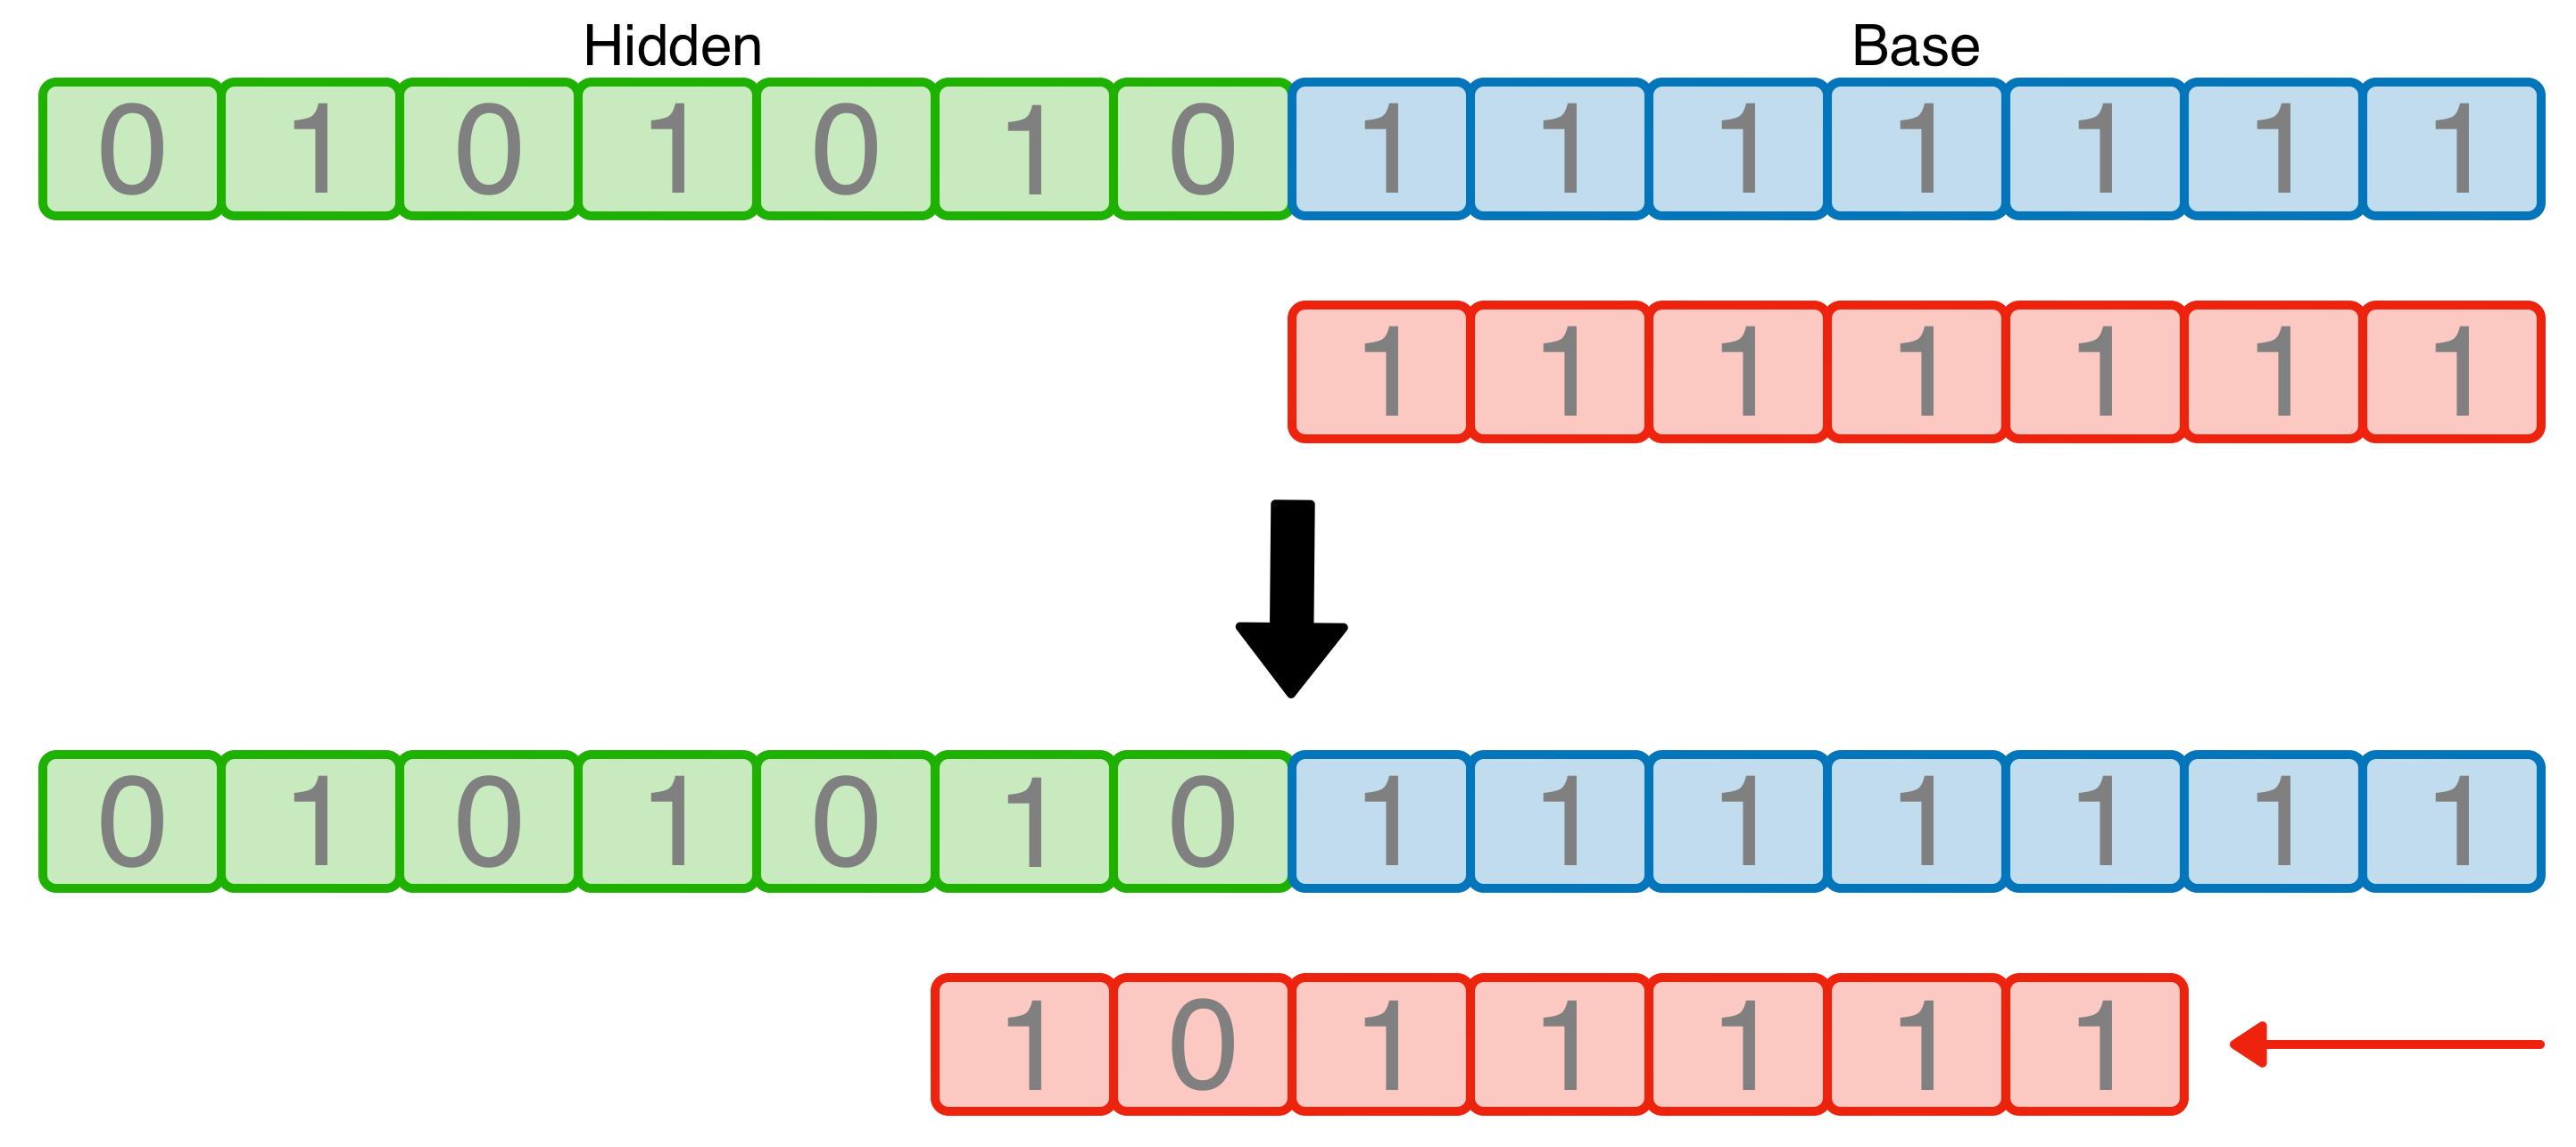
\includegraphics[width=0.75\textwidth]{gfx/ShiftRight.png}
    \begin{minipage}{0.49\textwidth}
        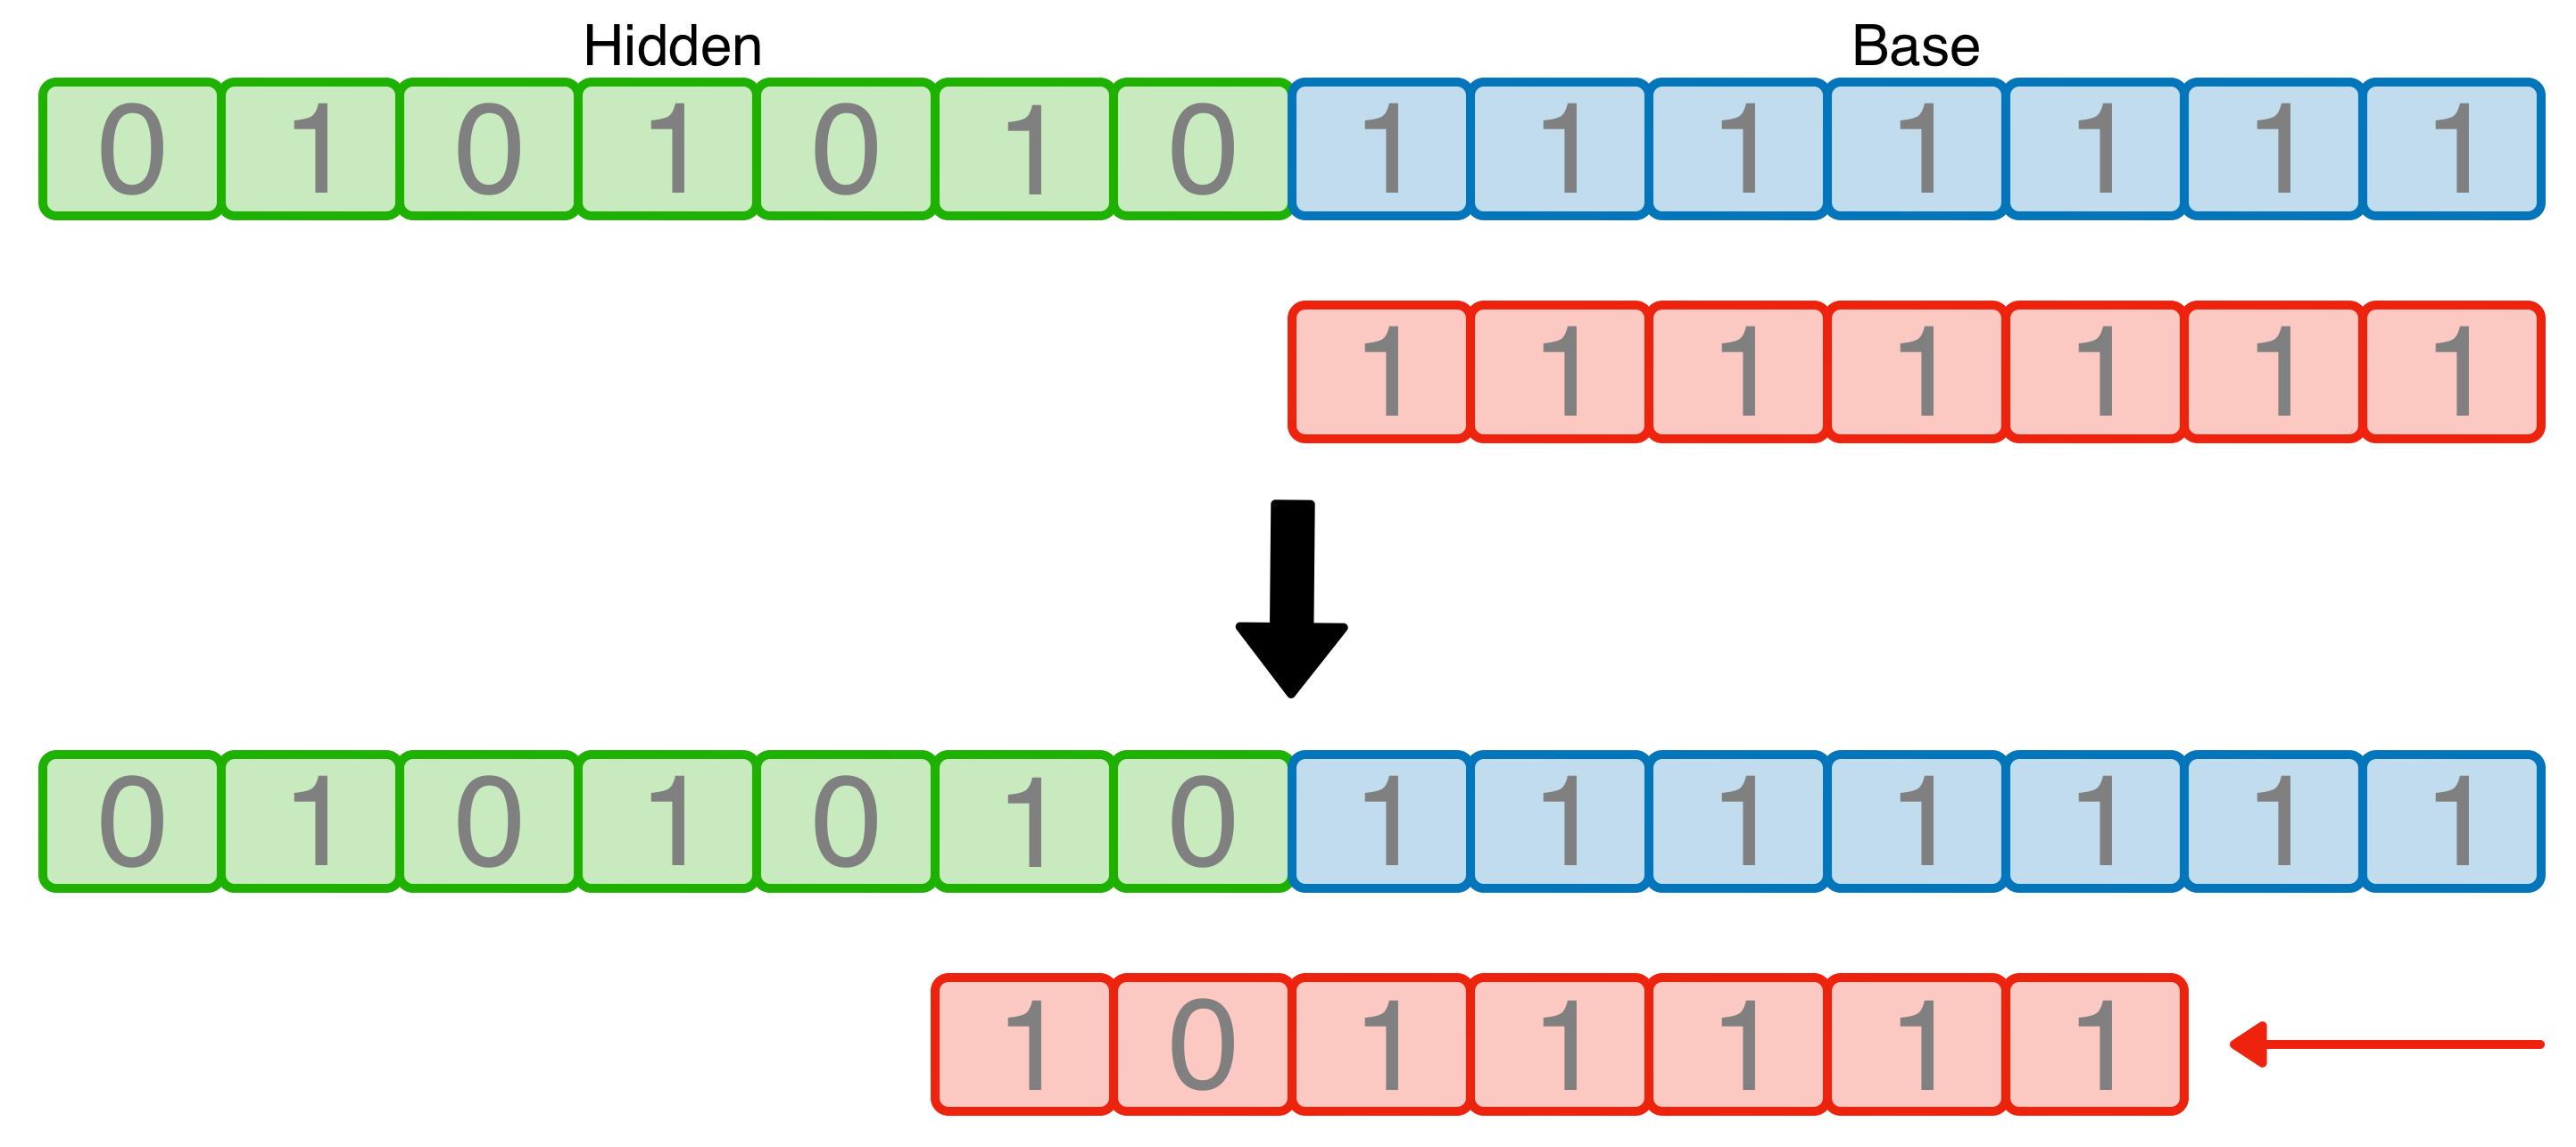
\includegraphics[width=\textwidth]{gfx/ShiftRight.png}
    \end{minipage}
    \hfill
    \begin{minipage}{0.49\textwidth}
        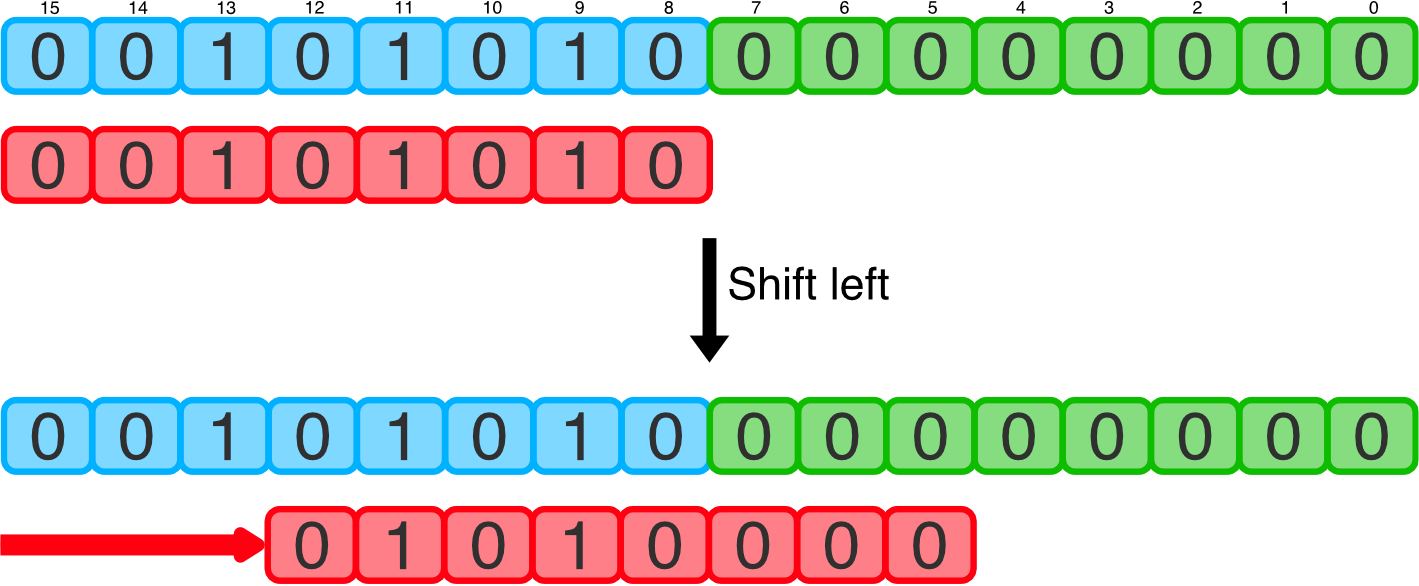
\includegraphics[width=\textwidth]{gfx/ShiftLeft.png}
    \end{minipage}
    \caption[A visual example of a right and a left shift.]{A visual example of a right shift by two, and a left shift by three. The green value represents the hidden value, the blue value represents the base value and the red value represents the value as visible.}
    \label{fig:shr}
\end{figure}

As we can see, this instruction is rather complex, and also transcends the conventional notion of shifts. Furthermore, the behavior of connecting signals and memory regions is not required at the IR level, but rather, it can be split in the frontend, resulting in operations acting on the two elements separately to obtain an equivalent behavior. For example, driving a connected signal is equivalent to driving the affected parts of the two signals separately, as illustrated in Figure \ref{fig:drvconn}.

\begin{figure}[ht]
    \centering
    \begin{minipage}{0.49\textwidth}
        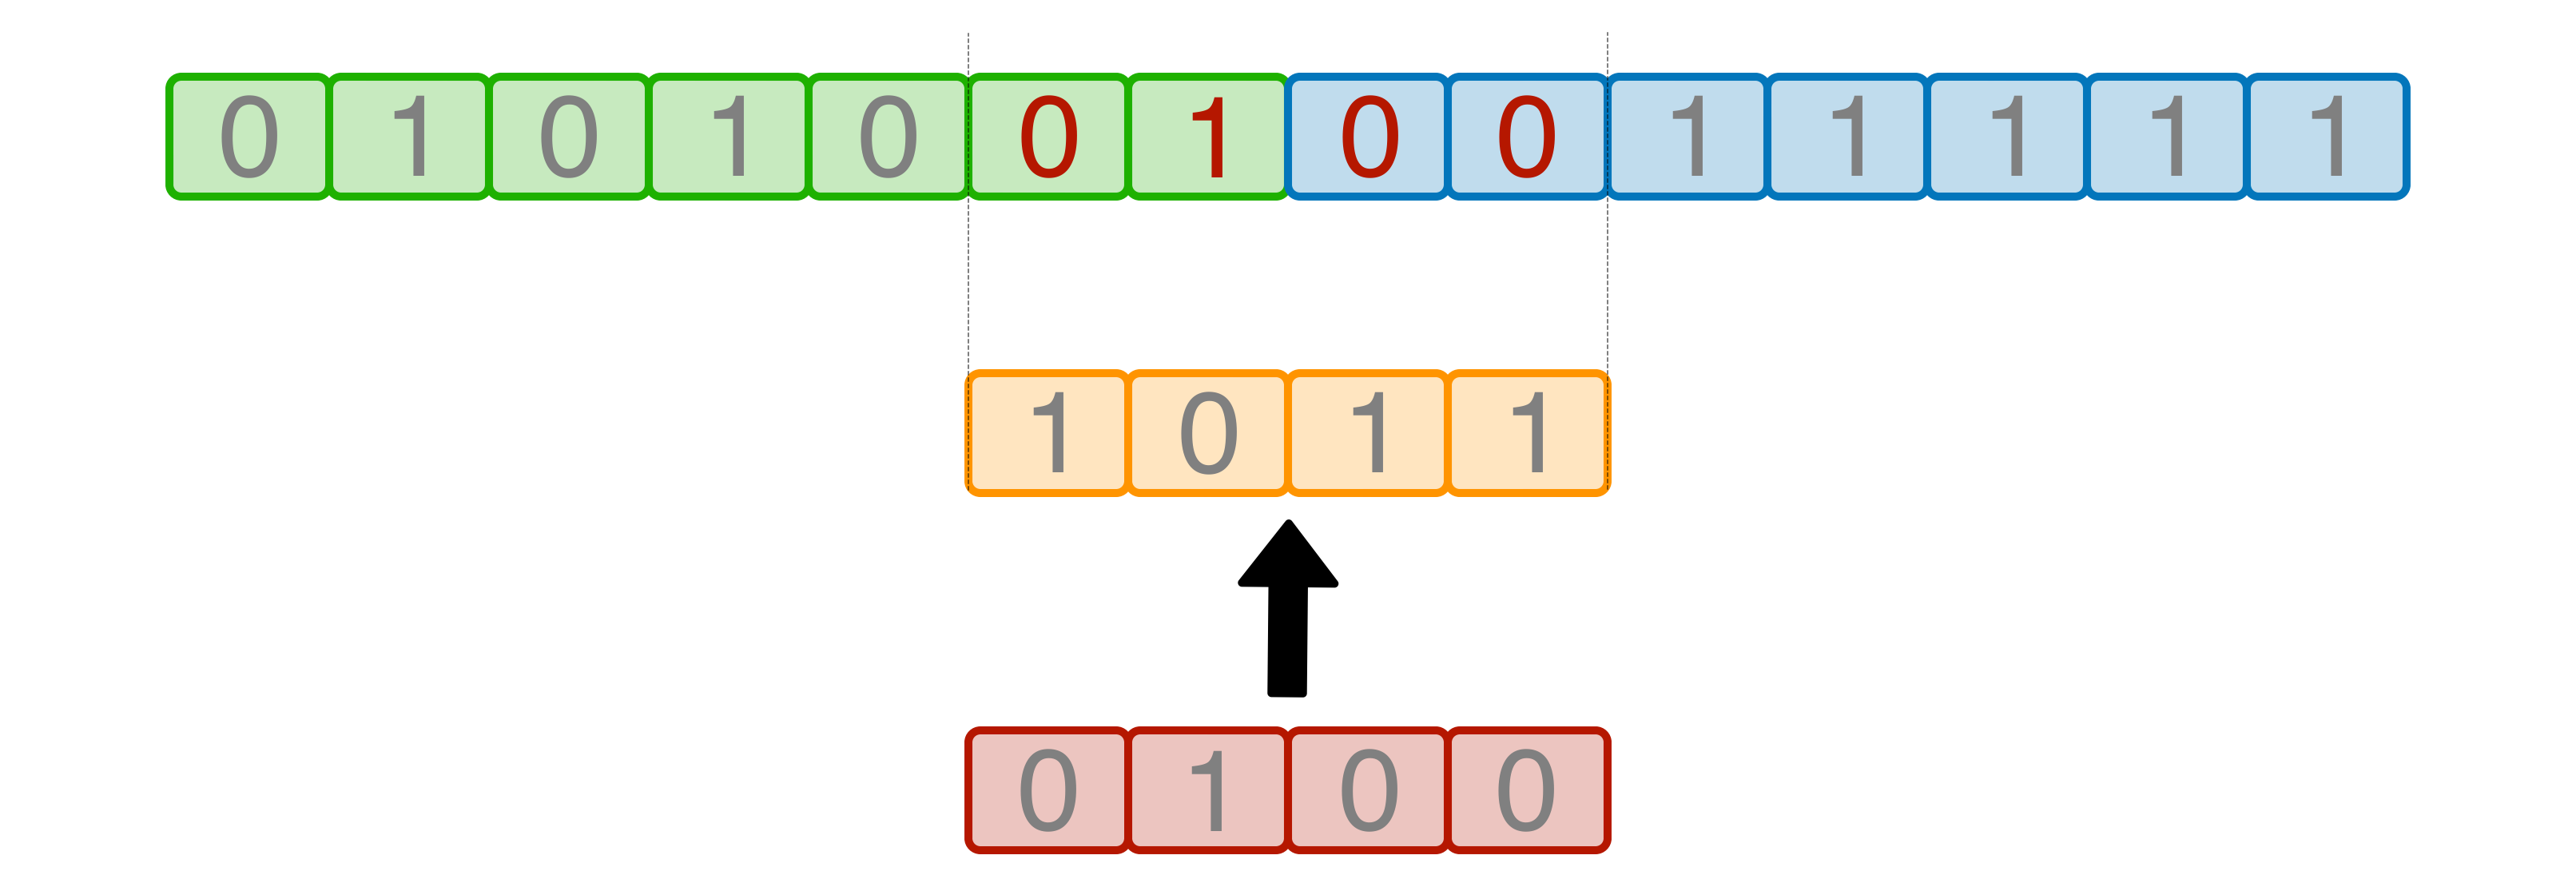
\includegraphics[width=\textwidth]{gfx/DrvConn.png}
    \end{minipage}
    \hfill
    \begin{minipage}{0.49\textwidth}
        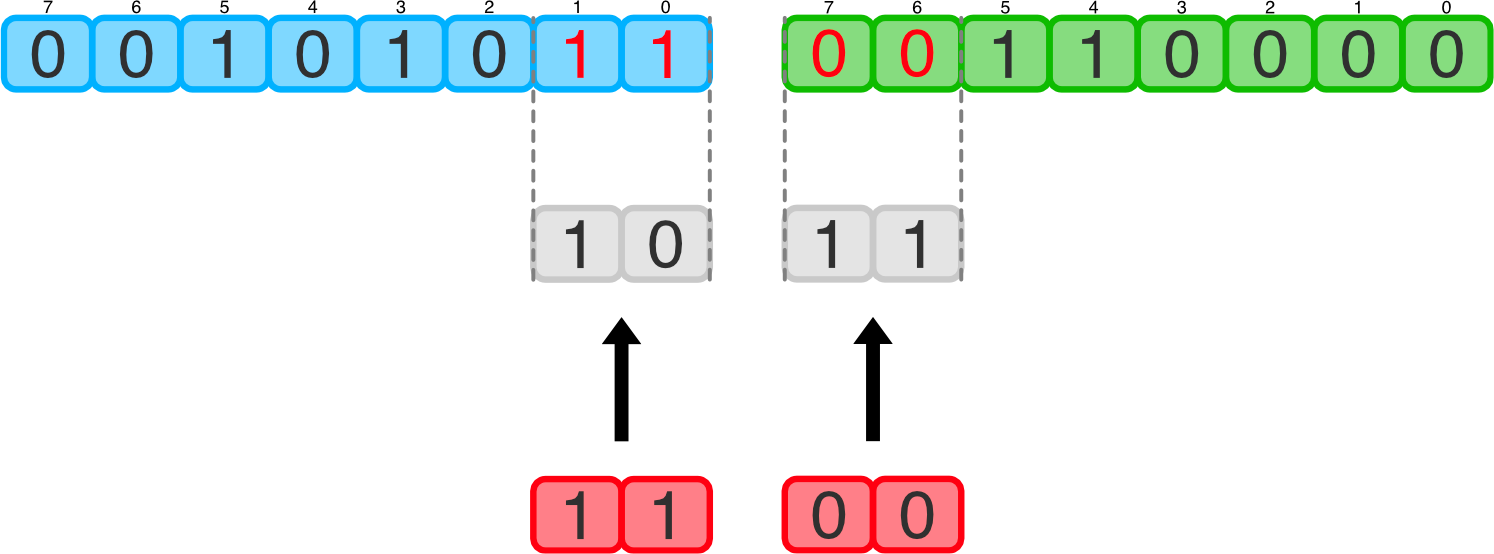
\includegraphics[width=\textwidth]{gfx/DrvSplit.png}
    \end{minipage}
    \caption[Illustration of driving a connected signal vs driving the two origin signals independently.]{Illustration of driving a connected signal and driving the two origin signals independently. The blue and green regions represent the two original signals, while the gray area represent their sub-signals. The red area and values represent the value to drive.}
    \label{fig:drvconn}
\end{figure}

To simplify the semantics of those instructions, we decided not to support shifting pointers and signals anymore, and to switch to conventional semantics for signed and unsigned shifts. Here we will require to include the respective new operations in the LLHD dialect, to support the logic types, though this has not been implemented yet. We thus still have the original LLHD shifting operations in our dialect, \texttt{llhd.shr} and \texttt{llhd.shl}, to fully support \texttt{moore}-generated code until the new semantics are fully adopted.

The LLHD shift instruction also enables to dynamically drive only parts of a signal, when the starting index of the slice (or element) is not known at compile time. We still need to be able to represent such behavior, for which we introduced a dynamic variant for the \textit{extract slice} and \textit{extract field} operations, described below.

\paragraph{Extraction and insertion operations}
LLHD provides extraction (and insertion) operations to extract (resp. insert) elements or slices from integers, arrays, and structs. Furthermore, the extraction operations are also defined on pointers and signals of such types, acting similarly to LLVM's \texttt{getelementptr} instruction and the shift instruction, as previously described. Namely, when used on signals and pointers, no value is probed (or loaded) from the respective signal (or memory location), instead, a new signal (or pointer) is created, pointing to the desired element (or the start of a slice).

Extraction and insertion operations come in two variants: \textit{extract element} and \textit{extract slice}. In our MLIR representation, each of those variants is represented by a different operation. Both take an attribute representing the index of the desired element (or the start of the slice) in the target value. This means they can only work when the start value is known at compile time. To work around this, \texttt{moore} commonly inserts first a shift, shifting the target value such that the desired index lands at the $0$-th position, and then extracts the desired value with index $0$.

Dynamic extraction, \ie, with a start index that is not statically known at compile-time, is very common in LLHD. LLHD's convoluted shift semantics are partially a consequence of this. To reduce the complexity of those operations, we introduced new dynamical extraction operations, aiming at eventually replacing those shift-and-extract patterns. An example of the new extraction operations can be found in Listing \ref{listing:extracts}, together with the static versions.

\mlirfile{An example of the extract operations.}{An example showing the syntax of the extract operations. The definitions of the various undefined operands are purposefully left out for readability.}{extracts}

\paragraph{Comparison operations}
MLIR provides a comparison operation for integers in the standard dialect, \texttt{cmpi}, which takes a predicate for the type of comparison to be executed (\eg equality or inequality). We use this operation for less-than and greater-than comparisons, but not the equality instructions. LLHD defines the \textit{equal} and \textit{not-equal} operations on all types, including structured types, where an element-wise comparison is performed, while the standard dialect's one is only defined for integers. We thus introduced a \texttt{llhd.eq} operation and a \texttt{llhd.neq} operation to cover the case of structured types comparison.
